\documentclass[a4paper, 12pt]{article}

\usepackage[T1]{fontenc}
\usepackage{IEEEtrantools}
\usepackage[]{amsmath}
\usepackage{amssymb}
\usepackage{float}
\usepackage[]{graphicx}
\usepackage{subfig}
\usepackage{caption}

\title{Control Systems: Practical 4}
\author{Ruan de Bruyn \and 216054484 \and Quintin Kruger \and 216008466}

\begin{document}

\pagenumbering{gobble}
\maketitle
\newpage
\pagenumbering{roman}
\tableofcontents
\listoffigures
\newpage
\pagenumbering{arabic}

\section{Introduction} % (fold)
\label{sec:introduction}
The purpose of this practical is to model discrete controllers using approximation methods to convert a continuous controller to a digital controller  and a more accurate approach where a complete digital design of the plant and controller is done. Used in this practical is a lead compensator defined by the equation that follows
\begin{equation}
	\label{eq:lead_compensator}
	D_c(s) = 
\end{equation}

<+DISCUSSION OF THE PLANT+>

<+DISCUSSION OF CONTINUOUS CONTROL ON PLANT+>
\begin{figure}[H]
  \centering
  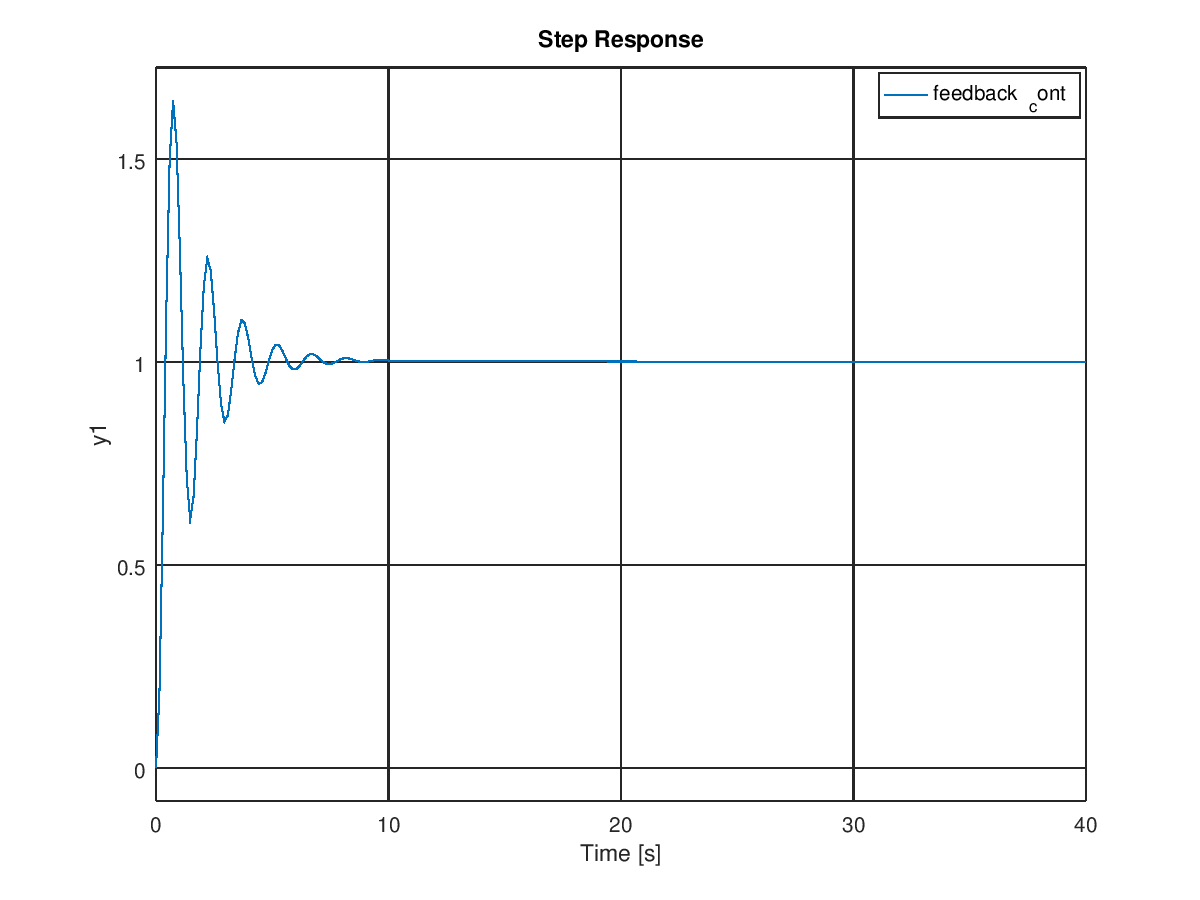
\includegraphics[width=\textwidth]{img/continuous_control.png}
  \caption{Continuous control using a lead compensator}
  \label{fig:continuous_control}
\end{figure}
% section introduction (end)

\section{Question 1} % (fold)
\label{sec:question_1}
The Tustin method of approximating the lead controller as defined by \eqref{eq:lead_compensator} was used to yield the discrete controller for the system in consideration. To follow are 4 different discrete controller results obtained for a number of different sampling times.

\begin{figure}[H]
  \centering
  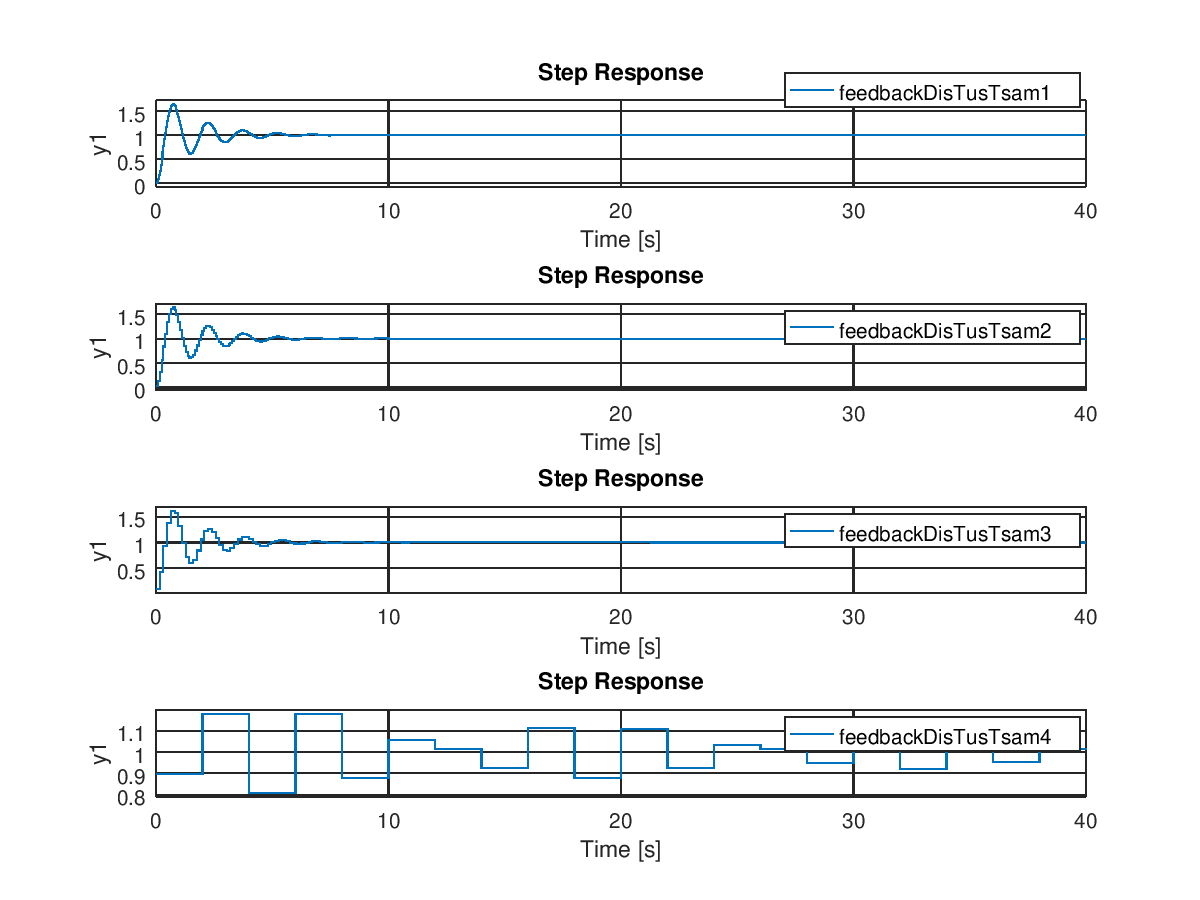
\includegraphics[width=\textwidth]{img/discrete_controllers.png}
  \caption{Discrete control of system using sample times of respectively 0.04, 0.08, 0.16 and 2 seconds}
  \label{fig:discrete_controllers}
\end{figure}

These plots were obtained by running the following octave code\\

  \noindent
  \texttt{plant = tf([5*9.8],[7 0 0]);}\\
  \texttt{plant\_dis\_tsam1 = c2d(plant,tsam1,'tustin');}\\
  \texttt{plant\_dis\_tsam2 = c2d(plant,tsam2,'tustin');}\\
  \texttt{plant\_dis\_tsam3 = c2d(plant,tsam3,'tustin');}\\
  \texttt{plant\_dis\_tsam4 = c2d(plant,tsam4,'tustin');}\\

  \noindent
  \texttt{cont\_cont = 0.28*tf([6.7 1],[0.106*6.7 1])}\\
  
  \noindent
  \texttt{feedback\_cont = feedback(plant*cont\_cont);}\\
  \texttt{figure;}\\
  \texttt{step(feedback\_cont)}\\
  
  \noindent
  \texttt{dis\_cont\_tus\_tsam1 = c2d(cont\_cont,tsam1,'tustin');}\\
  \texttt{dis\_cont\_tus\_tsam2 = c2d(cont\_cont,tsam2,'tustin');}\\
  \texttt{dis\_cont\_tus\_tsam3 = c2d(cont\_cont,tsam3,'tustin');}\\
  \texttt{dis\_cont\_tus\_tsam4 = c2d(cont\_cont,tsam4,'tustin');}\\
  
  \noindent
  \texttt{feedbackDisTusTsam1 = feedback(plant\_dis\_tsam1*dis\_cont\_tus\_tsam1);}\\
  \texttt{feedbackDisTusTsam2 = feedback(plant\_dis\_tsam2*dis\_cont\_tus\_tsam2);}\\
  \texttt{feedbackDisTusTsam3 = feedback(plant\_dis\_tsam3*dis\_cont\_tus\_tsam3);}\\
  \texttt{feedbackDisTusTsam4 = feedback(plant\_dis\_tsam4*dis\_cont\_tus\_tsam4);}\\
  
  \noindent
  \texttt{figure;}\\
  \texttt{subplot(4,1,1);}\\
  \texttt{step(feedbackDisTusTsam1)}\\
  \texttt{subplot(4,1,2);}\\
  \texttt{step(feedbackDisTusTsam2)}\\
  \texttt{subplot(4,1,3);}
  \texttt{step(feedbackDisTusTsam3)}\\
  \texttt{subplot(4,1,4);}\\
  \texttt{step(feedbackDisTusTsam4)}\\

The continuous system was made discrete in order to implement the feedback using the discrete controllers (another approach that would yield a better result is to use MATLAB's Simulink)\\

Now comparing these results with the application of the lead compensator, as dipicted in Figure \ref{fig:continuous_control}, we see that the best discrete approximation (that lies close to the step response of the continuously controlled system) is the Tustin discrete controller using a sampling time of $0.04$ seconds. As the sampling time increases (i.e. less samples are taken over the course of the same period) the approximation drifts off and the discrete controller doesn't provided the control that its continuous controller can provide (and should provide as the discrete controllers are approximations of the desired system response using a continuous controller).\\

The best sampling time yielding a close to exact replica of a system's response using a continuous controller is $20\times \omega_n$ where $\omega_n$ is the natural frequency of the system. Problems with the approximation come if the sampling time is chosen to be $10\times \omega_n$. It is safe to say that using a sampling time of $2$ seconds, is much less than $10\times \omega_n$ and sampling times of $0.04$, $0.08$ and $0.16$ lie closer to $20\times \omega_n$




% section question_1 (end)

\section{Question 2}

\begin{figure}[H]
	\centering
	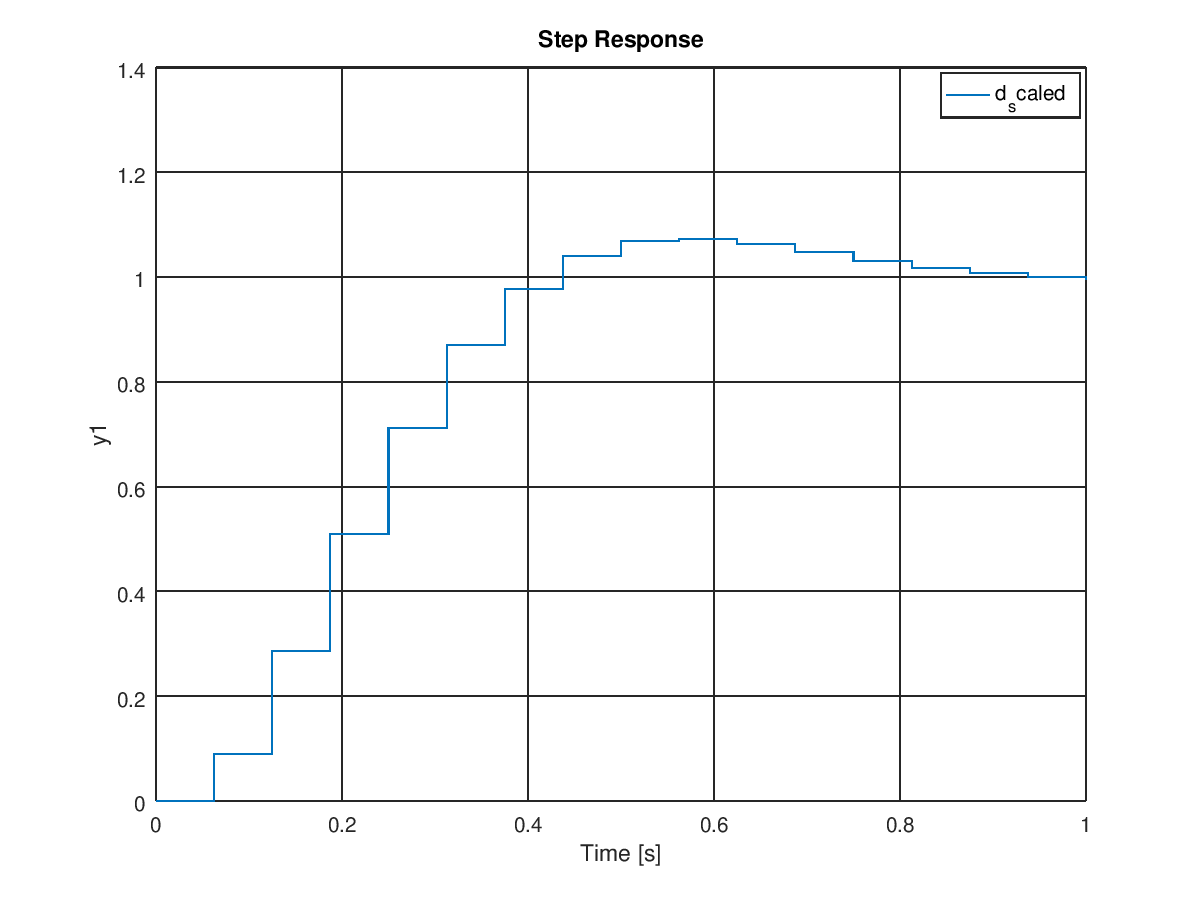
\includegraphics[width=\textwidth]{./img/2_1.png}
	\caption{ZOH system}
	\label{fig:2_1}
\end{figure}

Pole locations: -5 += 6j
Sampling time = 0.6s

% section question_2 (end)
\end{document}
